\documentclass[sigconf]{acmart}
\settopmatter{printacmref=false} % Removes citation information below abstract
\renewcommand\footnotetextcopyrightpermission[1]{} % removes footnote with conference information in first column
\pagestyle{plain} % removes running headers

\usepackage{listings}
\usepackage{booktabs} % For formal tables
\usepackage{multirow}
\usepackage{adjustbox}
%\usepackage[table,xcdraw]{xcolor}
\begin{document}
\begin{titlepage}
    
\Huge
Contribution Table
\vspace{0.5cm}

\begin{adjustbox}{width=\columnwidth}
    \begin{tabular}{||c c c c c c c||} 
         \hline
         Name & Maciej & Mohammad & Frederik & Abdirisaq & Alexander & Alberto \\ [0.4ex] 
         \hline\hline
         Abstract & 0\% & 100\%  & 0\%  & 0\%  & 0\%  & 0\% \\
         \hline
         Section 1 & 0\% & 10\%  & 90\%  & 0\%  & 0\%  & 0\% \\ 
         \hline
         Section 2 & 0\% & 0\%  & 0\%  & 0\%  & 0\%  & 100\% \\
         \hline
         Section 3 & 0\% & 17\%  & 10\%  & 56\%  & 0\%  & 17\% \\
         \hline
         Section 4 & 90\% & 5\%  & 5\%  & 0\%  & 0\%  & 0\% \\
         \hline
         Section 5 & 0\% & 0\%  & 0\%  & 0\%  & 100\%  & 0\% \\
         \hline
         Section 6 & 0\% & 0\%  & 75\%  & 25\%  & 0\%  & 0\% \\
         \hline
         Section 7 & 0\% & 50\%  & 0\%  & 0\%  & 0\%  & 50\% \\
        \hline
         Code & 60\% & 12\%  & 12\%  & 12\%  & 2\%  & 2\% \\
         \hline
         Experiments & 10\% & 5\%  & 5\%  & 5\%  & 70\%  & 5\% \\
        \hline
    \end{tabular}
\end{adjustbox}
\end{titlepage}

\title{Preventing Phantom Traffic with V2V Communication and Autonomous Driving}
\subtitle{02223 MBSE final project}


\author{Mohammad Nabil Ahmad}
\affiliation{%
}
\email{s184355@student.dtu.dk}
\author{Frederik Schibelfeldt}
\affiliation{%
}
\email{s184477@student.dtu.dk}
\author{Abdirisaq Farah}
\affiliation{%
}
\email{s163157@student.dtu.dk}

\author{Maciej Tatarski}
\affiliation{%
}
\email{s202609@student.dtu.dk}
\author{Alexander Welsch Carlsen}
\affiliation{%
}
\email{s200463@student.dtu.dk}
\author{Alberto Raheli}
\affiliation{%
}
\email{s211012@student.dtu.dk}
\begin{abstract}
In this study, an intelligent vehicle that is autonomously controlled is introduced in a highway model with a traffic inflow where phantom traffic congestion occurs. The autonomously controlled vehicles implement a V2V communication system that shares information on speed and position of each autonomous vehicle along with the direction of the vehicles. The behavior of autonomous vehicles is ideal compared to human-driven vehicles thus the acceleration and breaking aim to prevent phantom traffic jams. Based on the ratio between the autonomous vehicles and human-driven vehicles the results shows that with 60\% of autonomous vehicles the flow of vehicles passing the highway is doubled compared to no autonomous vehicles. With 80\% of autonomous vehicles, the flow almost reaches the upper limit only increasing slightly if the autonomous vehicles parameter is brought up to 100\%.
\end{abstract}
\maketitle

% \renewcommand{\shortauthors}{DTU}
% \acmConference[MBSE]{MBSE}{December 2021}{Copenhagen, DK}

% Insert sections here
\section{Introduction }
The increase in greenhouse gas emissions, contributed by a high volume of traffic along with traffic jams, continues to increase every year except for these recent years due to the COVID-19 pandemic. However, in cities such as New York, a driver would still spend around 100 hours extra due to congestion\cite{TrafficReport}, thus increasing emissions of greenhouse gasses and increasing the cost of transportation for the driver.

There are several proposed approaches to help reduce traffic in cities with recurring traffic jams, and one of these approaches is to use vehicle to vehicle (V2V) communication along with autonomous vehicles. These are two technologies that are in constant development and the complexity of these systems increase year after year.

These technologies allow cities to more efficiently use the current infrastructure instead of expanding on their current road network.

This report aims to answer whether or not autonomous vehicles using vehicle to vehicle communication can reduce traffic in cities with recurring traffic jams. This is done by creating a model of a simple highway system with several vehicles in it, and simulating a base case of regular vehicles against different proportions of vehicles implementing these technologies.

The report will be structured in sections and each section can be described as follows: 
% put this in itemize
\begin{itemize}
    \item Section 2 will introduce some of the concepts and the problem statement for this report.
    \item Section 3 will discuss the proposed model that was used to create the simulations
    \item Section 4 will discuss how this model was implemented along with the visualization of the simulations.
    \item Section 5 will analyze the simulations that were conducted and discuss the different experiments.
    \item Section 6 and 7 will conclude the report, with a discussion about the results and future work to be done to the model and simulator along with a short conclusion to the report.
\end{itemize}
\section{Problem Statement}
\label{sec:problem-statement}
This section is focused on exploring the challenges of reducing and preventing traffic using vehicle to vehicle (V2V) communication and autonomous driving.
\subsection{Phantom Traffic}
Traffic can occur for multiple reason and for this project a specific type, called \textit{phantom traffic}, was considered. Is one of the most common and more complex form of traffic as is not due to something concrete like an accidents or a traffic lights. It occurs when a lot of cars are on the roads at the same time and just a simple disturbance in the flow can create a ripple effect that generates the congestion. Even a common maneuver like lane changing, if poorly executed, can lead to serious traffic jam \cite{Phantom}.

In essence phantom traffic is caused by the imperfection of the human being, by its relatively low reaction time and its limited perception of the space around itself. For this reason it was questioned if in order to solve congestion the solution could be to remove the human factor from the equation and let computers handle decisions on the road.
\subsection{V2V Communication and Car Automation}
An autonomous car by itself could probably help reduce traffic using sensors, cameras and technologies like adaptive cruise control\cite{ACC} but for this project it was decided to address the problem through the additional implementation of a wireless communication network inspired by the Vehicle-to-vehicle (V2V) communication paradigm \cite{V2V}. V2V communication consists of a network specifically designed for vehicles that allows the sharing of real time information including data like velocity, position, acceleration and general status of the car. 

With this kind of information the technological upgrade to an autonomous car capable of making it own decisions based not only to sensors but also on the received information from other cars would not only be easily achievable but would also lead to improve the efficiency of an autonomous car\cite{V2Vimprovement}. 

\subsection{Question}
This project will try to demonstrate that a system that combine V2V communication and car automation would allow each autonomous car to know in advance what is happening further down the road and react with much more efficiency than a human. This paper is going to discuss if, in a scenario with recurrent congestion due to phantom traffic, it is possible to increase vehicle flow and also what proportion of autonomous connected cars would be needed.





\section{Methodology}
\label{sec:section3}
 
The aim in the study is to investigate what effects autonomous cars using vehicle to vehicle (V2V) communication have on traffic. The methodology technique chosen to investigate the presented problem stated in \hyperref[sec:problem-statement]{section 2} is presented in the following. This will be done by firstly discussing the proposed microscopic model. Thereafter we present the environment of the model. Finally, we discuss the modelling of the human behaviour and the effect a driver's mood has on the surroundings \& environment. 
\subsection{Model}
The aim of the presented model is to allow us to analyse the effects of the different proportions on the highway flow.  Furthermore, we analyse the the inflow and the average velocity of the cars in the environment. \\
\\
The proposed model is a microscopic model meaning that we represent the vehicles \& their behavior separately. The different  behavioral aspects range from speed, acceleration, lane changing \& gap acceptance. 
The model consists of three types of vehicles, cars autonomous cars \& trucks. Each of three vehicles are separate entities that react on received input from the environment.The Three types of vehicles proposed in the model are discussed in more detail in the following. \\ 
\\ 
The first type being the type car, which is considered a regular vehicle, where the driver affects decision-making. This means that it is only the driver that decides the course of action for the vehicle. The driver observes the environment \& has a mood attribute that determines how likely he is to react to surroundings such as a car slowing down. \\
The second type of vehicle in the model is the truck. The decision making for a truck is made by the driver and only the driver, the same as with the car type, however with the crucial difference of having a lower speed limit \& more consciousness driver behavior. This means, that Trucks are more likely to stay on the most right lane, less likely to overtake \& less likely to react to the environment. \\
As for the third type of vehicle it is the autonomous car. The autonomous car as opposed to the two aforementioned types derives its decision making from two components. The first of these components is the driver \& the second is the V2V communication received from both other autonomous cars \& the environment. The driver input in the autonomous car is weighted lower than decision making that is dependent on the V2V communication received. The V2V communication refers to the communication from the environment as the autonomous cars communicate  with other autonomous cars on the highway. The driver behavior aspects of the three presented vehicles is discussed in further detail in the \hyperref[HumanBehaviour]{human behaviour} subsection.\\ 
\\
The model aims to model the real-life phenomena of phantom traffic \& the driver reactions effect on traffic jams. As discussed in the phantom traffic section a disturbance in the traffic flow \& reaction times are the main causes of traffic slow down. Thus, it is essential for the model to be able to replicate how a driver reacts to such a scenario, thus the Intelligent Driver Model (IDM) was selected allowing for a more accurate driver behaviour. \cite{CaoIDM}
% 



% ---------------- BELOW CAN BE USED FOR ENV ---------------------------------

% The modeling of the traffic flow is based on a set in of input parameters. 
%These input parameters will be shortly presented in the fl 
% The first of these parameters is the inflow. The inflow parameter indicates the ratio of vehicle spawning at the entry lanes of the highway and allows for generation of various degrees \& forms of phantom traffic. The second parameter is the proportion of autonomous cars, which indicates the proportion of the inflow that is auto cars. The third parameter of the traffic flow model is the proportion of trucks. Trucks are similarly to cars however with the crucial difference of having a lower speed limit & more consciousness driver behavior.
 

%Furthermore, we allow for the tweaking of the behaviour of the driver as 

%-

\subsection{Environment}
As stated in the introduction section, the model proposed in this report consists of a highway environment wherein the traffic flow of various types of vehicles is modelled. The highway consists of multiple lanes. The basis of the highway is defined by a length and a speed limit. The length of the highway defined in meters is used as an one of the evaluation criteria for the number of vehicles passing the highway. The speed limit defined in kilometers per hour which defines an upper limit for the speed of the vehicles. Likewise, the average speed of the vehicles is used as an evaluation criteria. The greater number of cars passing the highway and the higher average speed of the vehicles generally indicates less phantom traffic congestion.\\
Studies shows various methods of defining traffic density. \cite{YANG2017344} For the environment model the traffic inflow is defined as the number of cars spawning at the beginning of the highway. 

\subsection{Human behaviour}
\label{HumanBehaviour}
The human behavior was modeled by giving each driver a possibility to do a range of actions same as a driver in the real world could do. These actions are the basic actions that a driver in the real world could do, such as accelerating, braking or changing lanes. To model the human behaviour, each driver is able to do each of these actions and decide what action do depending on the driver surrounding environment. Similar to a real life situation, a driver can only do actions depending on the surrounding environment, as a driver has no knowledge of what is happening outside of their own bubble. 

Each driver was given a random 'mood', this mood decides how likely it is for a driver to do an action. This addresses the fact that there are more aggressive drivers than others. This means that if a driver has a high mood, the driver is more likely to do actions such as accelerating, changing lanes and so fourth. 
The drivers were modeled to follow regular driving behaviours such as trying to keep to the right if possible, and also to go as close to the speed limit as possible. If a driver sees that it will collide with the car in front, the driver has two decisions it can make, either change lane if possible, or brake to avoid hitting the vehicle in front. 

This behaviour is what causes the traffic jams, since the driver has no knowledge of the decision that the drivers in front of them are going to make, but can only make decisions based on what they can currently observe.\cite{HumanBehaviour}

\subsection{Assumption}
For the simulation it has been chosen to work in an hypothetical highway environment. This assumption give an initial constraint to the grate level of complexity that a road system can easily reach, however it was necessary to limit the scope of our project. Moreover it gave us the opportunity to focus on producing actual result with the simulator in an environment that, even if simplified, is one of the most used by drivers all around the word and where phantom traffic jams are very common.

Other assumptions regard the communication between vehicles. The V2V communication system is a well defined paradigm that we only take as a baseline in our model. We assume that all the information that a car receive from the others can be used by the vehicles in our simulation to make autonomous decision that take action on the existing drive train of the car. 
Moreover in this first iteration of the simulator it is also assumed that the communication between vehicles happens without delays or errors. 
\section{Implementation}
Simulation, as well as visualization, was implemented in python using object oriented programming paradigm, all elements are kept in a single repository on GitHub\cite{repository}. It was crucial for the project to separate those entities to ensure seamless testing possibilities as well as recreating animation from previously performed simulations. For testing purposes simulation can also be run using multi-threading, taking input from standard input, in particular test files with specified parameters of the simulations. It makes plotting and testing faster as simulations with many cars can be time-intensive.

\subsection{Simulation}
Simulation is a part of the project which produces specific output from given parameters, imitating real-world behavior. All classes implemented can be seen on a diagram in appendix \ref{appendix:classDiagram}. The main class responsible for performing the simulation is a Scheduler class. It is taking several parameters as an input which can be seen below:

\begin{itemize}
    \item Average driver mood
    \item Number of lanes
    \item Entry lane attributes
    \item Highway length [km]
    \item Speed limit [km/h]
    \item Proportion of Autonomous cars
    \item Proportion of Trucks
\end{itemize}

An instance of this class is storing the mentioned parameters as constants for the simulation and propagating them to all subordinate classes. All parameters given are being translated to SI units before propagation. In the initial architecture, it was decided to make a fixed time step in the simulation, equal to one second.

When initialized, the scheduler creates an instance of the Highway class with a given number of Lanes instances, speed limit, length, and other properties. This object will later be used to render the simulation.

There are two options to perform simulations, either manual or automatic. The former can be used to create a specific simulation with full control over the state and object. It requires manually calling the step function which is updating the simulation. The advantage of this option is that all parameters can be changed in between the steps but it also requires a lot of manual labor and steps.

The automatic simulation takes two arguments to be able to perform actions: Inflow [vehicle/minute], Simulation time [s]. After being called, it is performing several steps equal to the simulation time. In between steps, the scheduler is deciding if and where to spawn the vehicles to achieve set inflow on a highway. Every action involved in a simulation and a step function can be seen in figure \ref{fig:sim-steps}.

\begin{figure}[H]
    \centering
    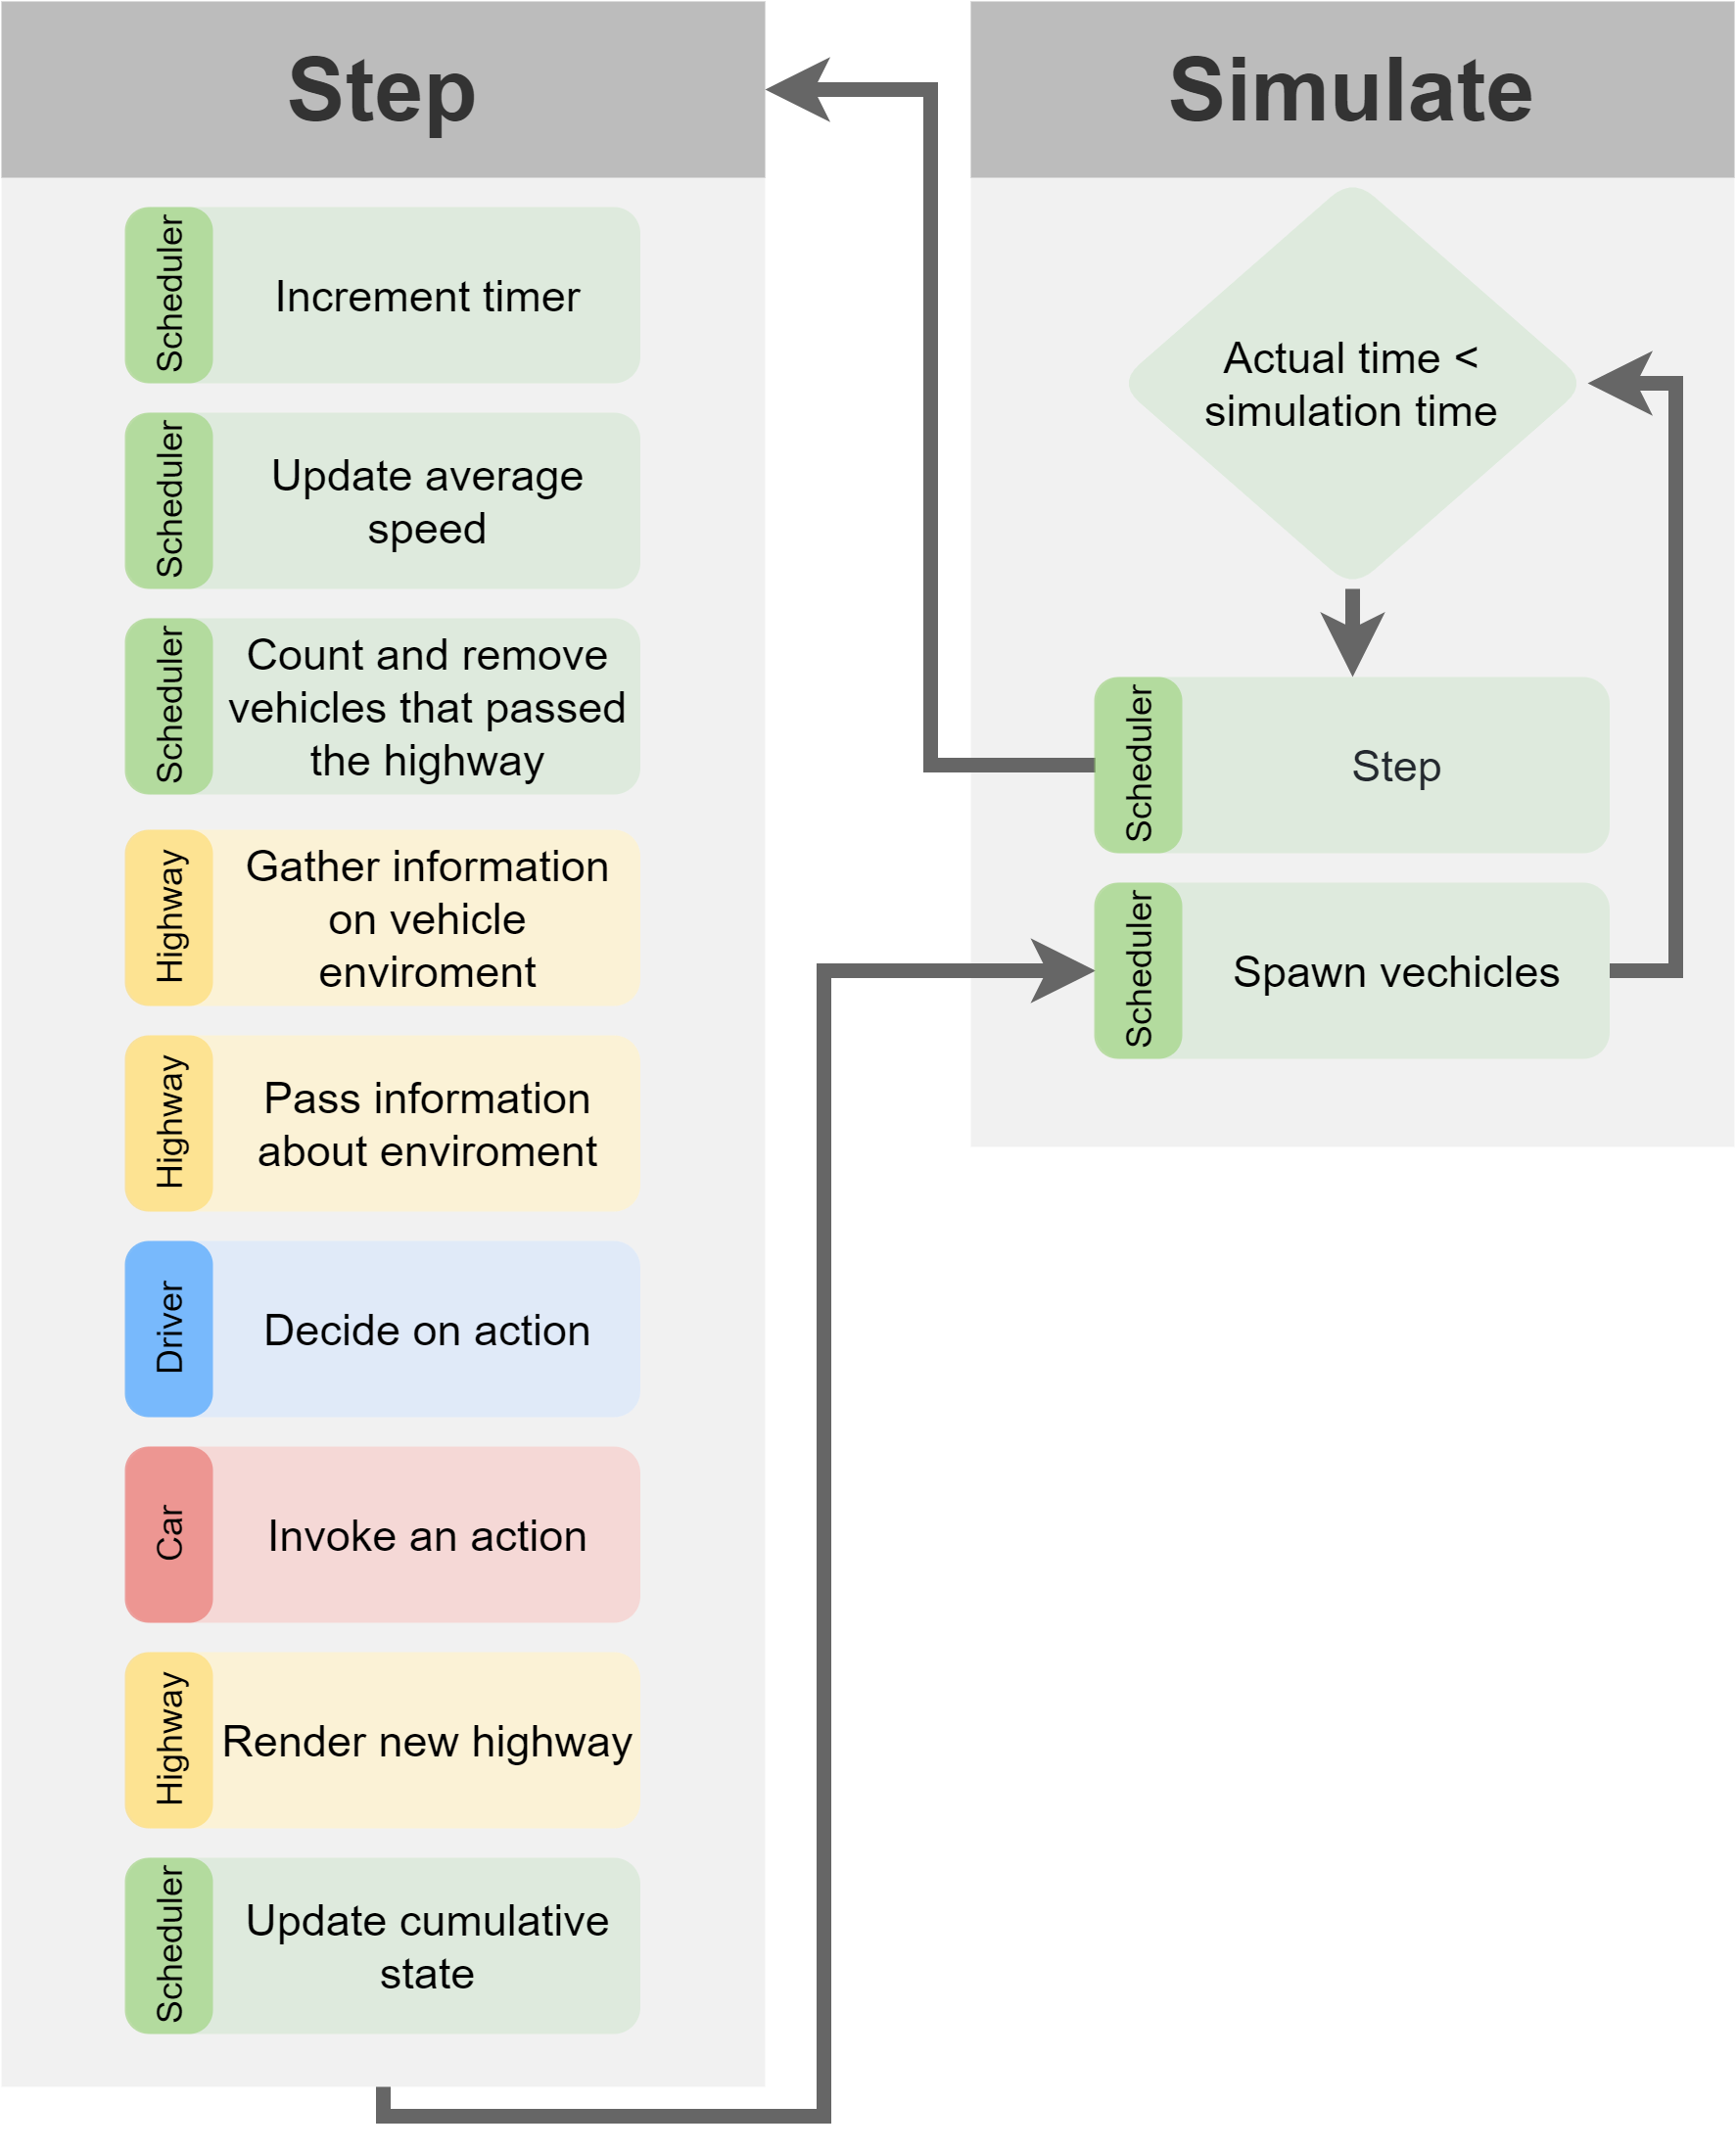
\includegraphics[width= \linewidth]{images/simulation-steps.png}
    \caption{Logic behind simulation.}
    \label{fig:sim-steps}
\end{figure}

To generate the vehicles, the scheduler is choosing between spawning different types of vehicles( Car, Truck or Autonomous car) with the probabilities given as a desired proportion of the vehicles on a final Highway object where:

\begin{multline}
    \begin{gathered}
        {P(autonomous\ car)}=proportion\ of\ autonomous\\
        {P(truck)}=proportion\ of\ truck\\
        {P(car)}=1-proportion\ of\ truck\ - proportion\ of\ truck
    \end{gathered}
\end{multline}

For Car and Autonomous car, the speed of the vehicle is being chosen from a normal distribution in relation to the speed limit on a highway:

\begin{multline}
  vehicle\ speed = \mathcal{N}(speed\ limit,\,(0.1*speed\ limit)^{2})
\end{multline}

To make the simulation easily extensible by adding new types of vehicles polymorphism and inheritance were introduced. Any type of vehicle can inherit from the Car class and change the behavior by setting different parameters and overloading take action method(figure \ref{fig:polymorphism}), f.e Autonomous car is taking an action not only based on the driver's decision but also it's own knowledge about the environment. For now, there are three vehicles types implemented: Truck - slow, and not willing to take many actions, Autonomous car - an entity that considers the position and speed of the other autonomous cars to decide on an action, Car - normal car vehicle, controlled by a driver. Every vehicle includes a Driver class instance as a parameter and invokes an action based on its decisions and in some cases additional knowledge(Autonomous car).

\begin{figure}[H]
    \centering
    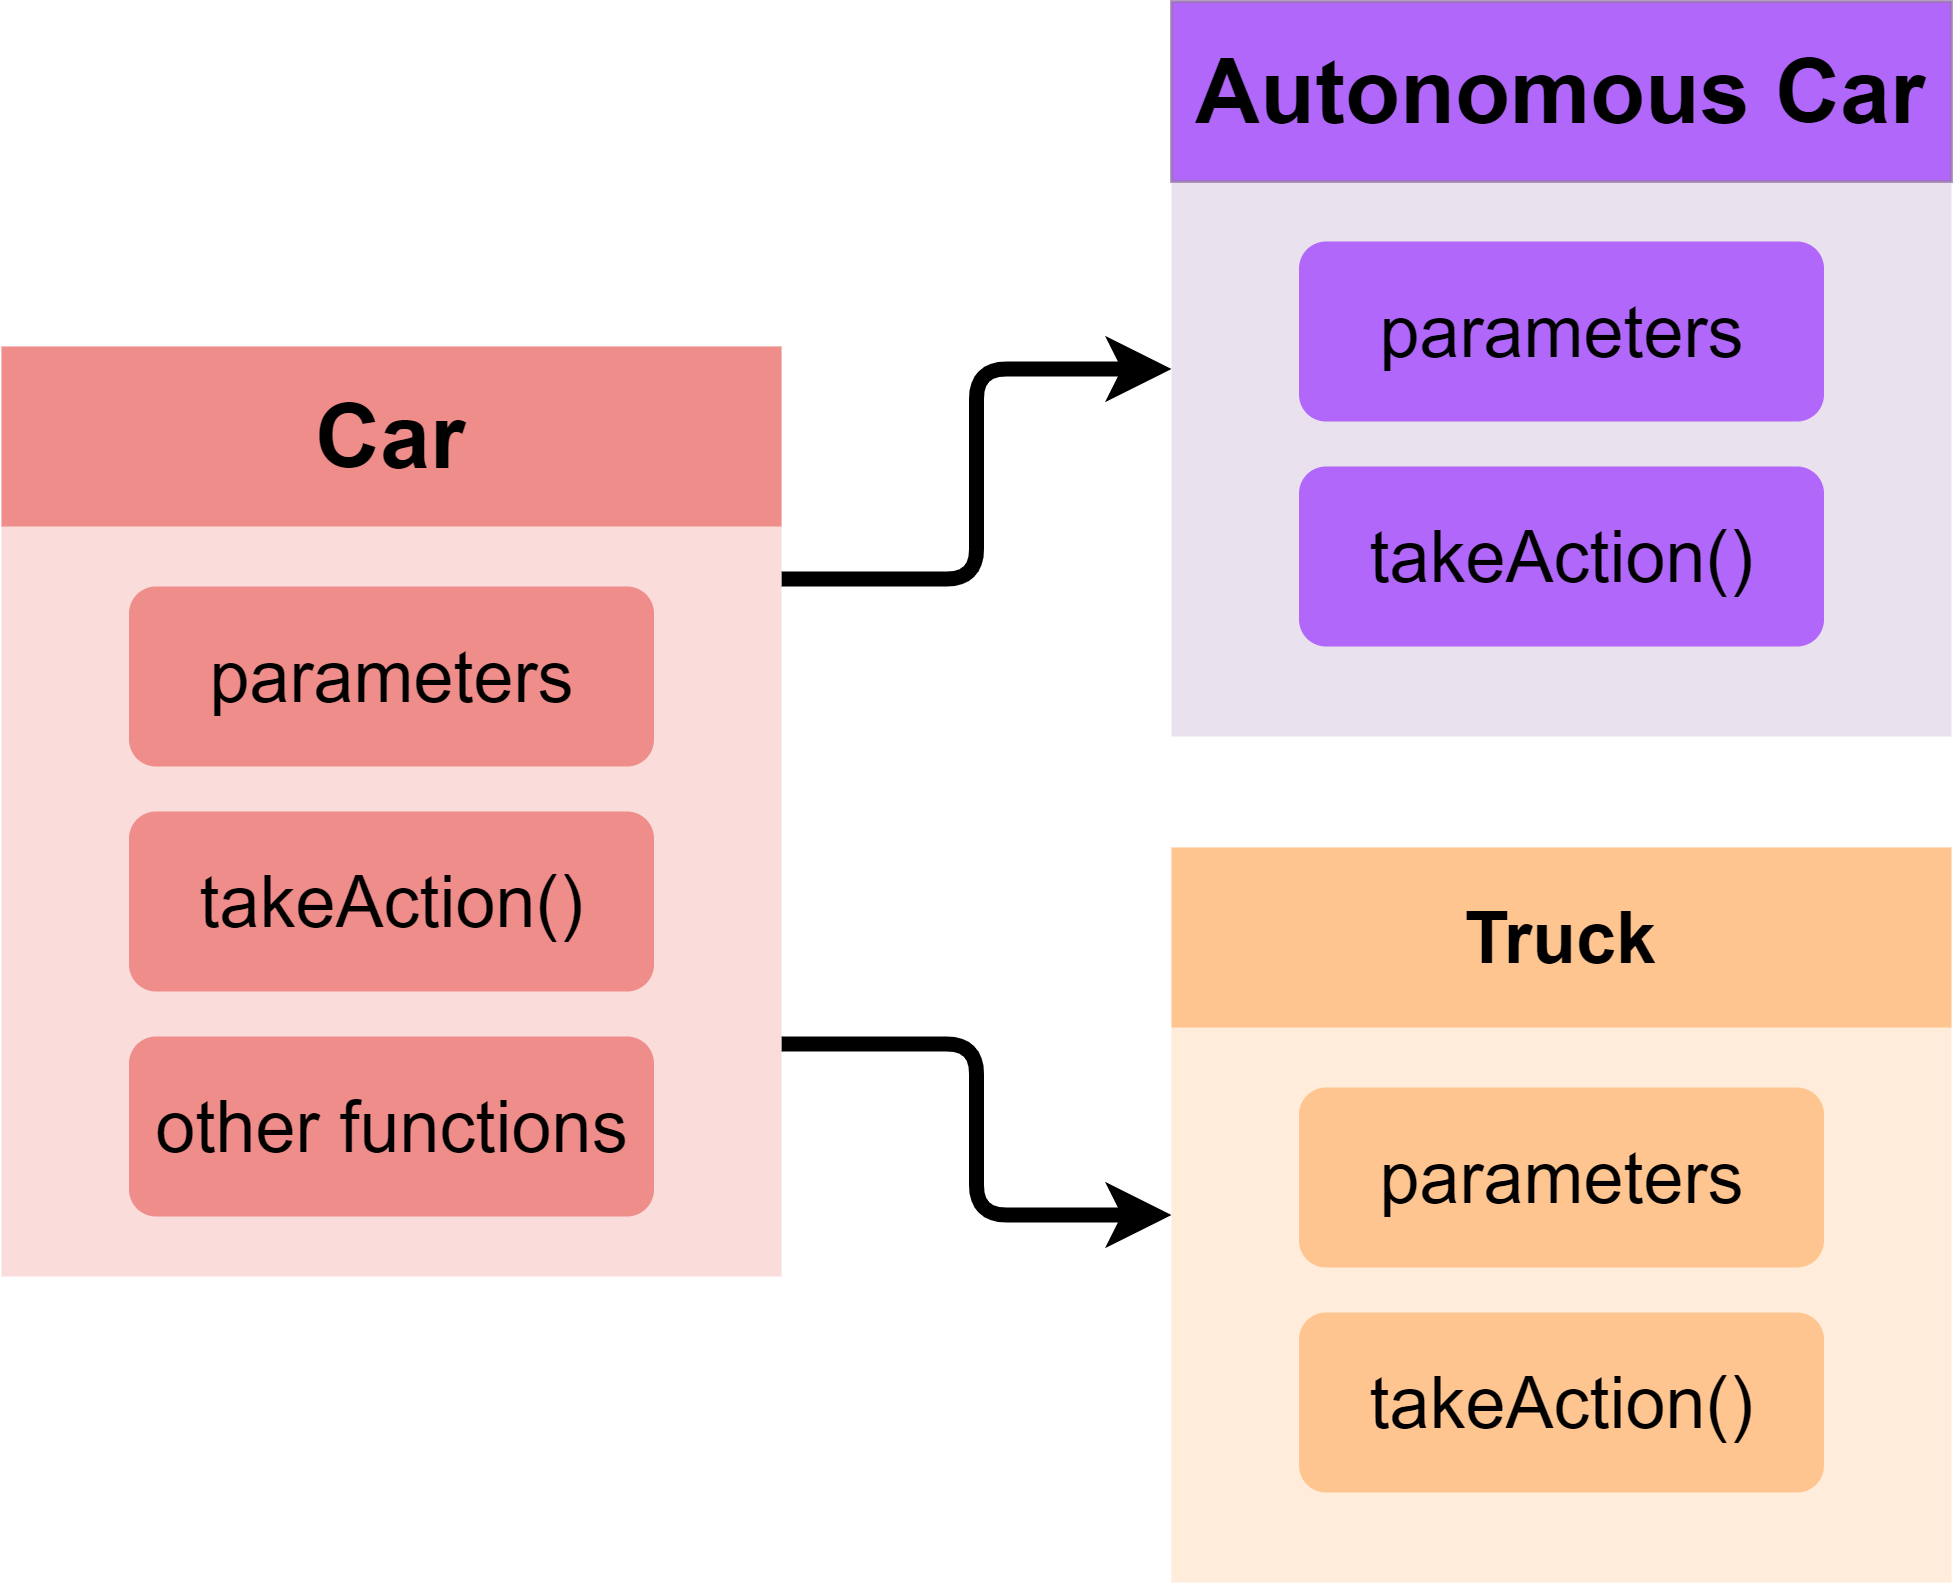
\includegraphics[width=0.9\linewidth]{images/polymorphism.png}
    \caption{Logic of polymorphism.}
    \label{fig:polymorphism}
\end{figure}

Additional capabilities of the simulation:
\begin{itemize}
    \item Exporting state to JSON file.
    \item Exporting the whole scheduler to a pickle file.
    \item Importing both state and scheduler from the file.
    \item Resetting scheduler state to build a new simulation with the same parameters.
\end{itemize}

\subsection{Visualization}
It was decided to make a simple visualization based on pythons matplotlib library\cite{Hunter:2007}, more specifically its animation function. As visualization is completely separated from simulation it can directly take the dictionary generated by simulation or fetch the input from a valid JSON file. Validity means that it has to follow a certain structure(as generated from the scheduler class), presented in the appendix \ref{appendix:json-schema}.

The visualization module is then plotting each step of the simulation as one frame of the final animation, where the x-axis represents the distance from the beginning of the highway and the y-axis represents the lane. Cars are being colored in relation to their unique id, there is also an option to color them based on the class of the vehicle which can be seen in appendix \ref{appendix:color-output}. The outcome can be presented interactively as a matplotlib plot or exported to a GIF file, the latter usually works better as it is more smooth. Representation of a single highway with 5 lanes can be seen in figure \ref{fig:single-highway}, color coding is based on the unique id of a car.

\begin{figure}[H]
    \centering
    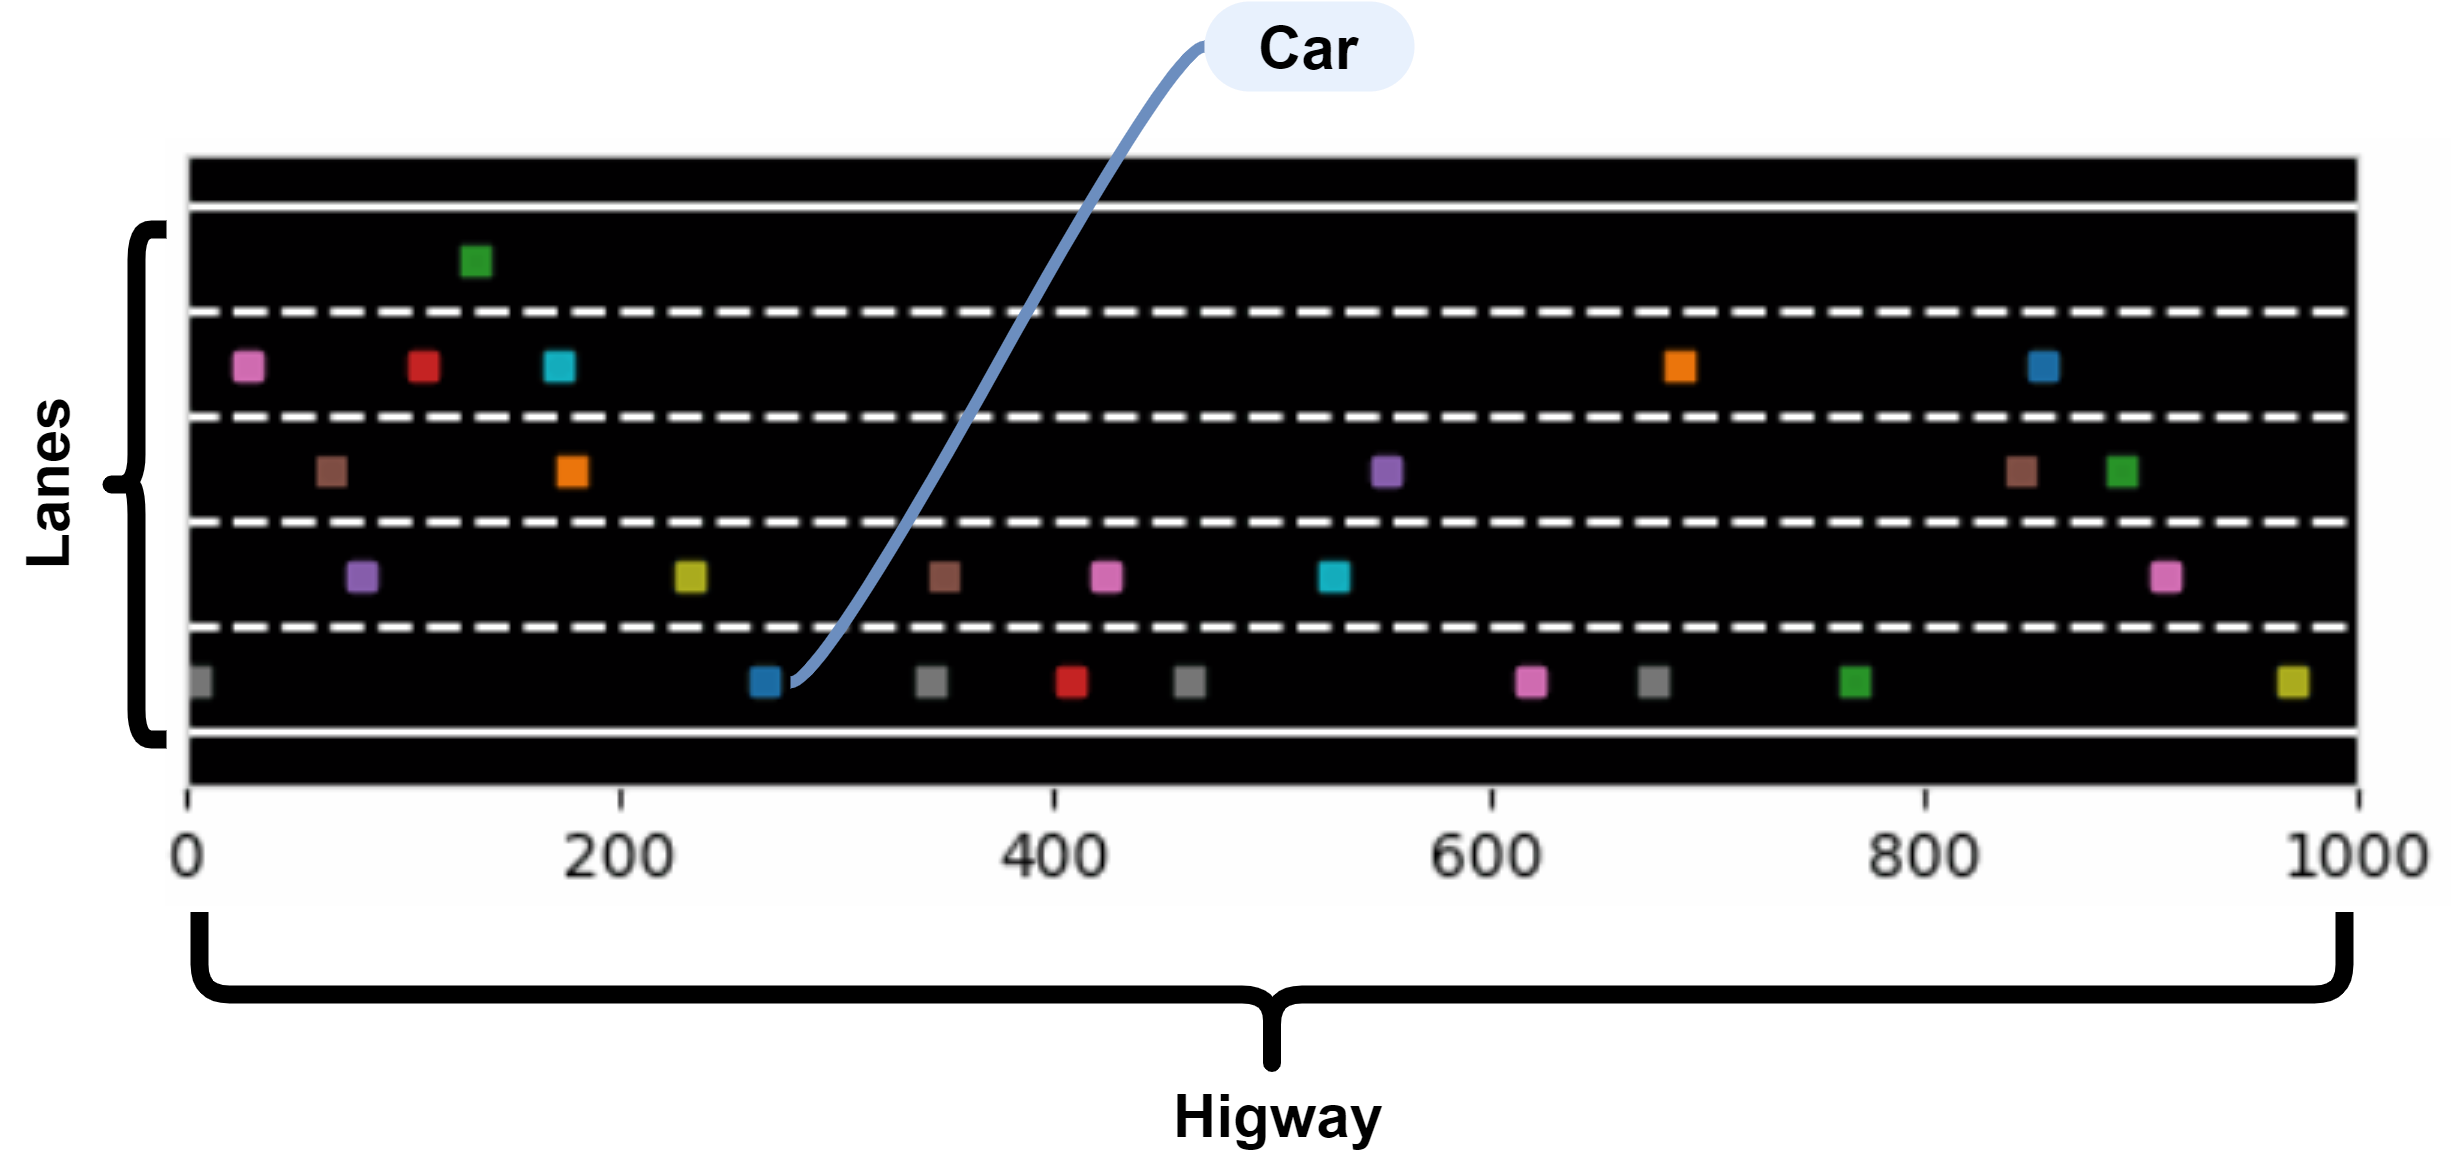
\includegraphics[width=\linewidth]{images/single-highwa.png}
    \caption{Single highway animation.}
    \label{fig:single-highway}
\end{figure}

Visualization can be made from multiple simulations with different parameters, and it is automatically adjusting all plots, additionally, the speed of the simulation can be adjusted by tweaking two parameters: data reduction and animation speed. Results from the simulation can be seen in real-time in form of a bar plot that indicates current vehicle flow on the highway and a line plot that shows average speed on each simulation. 

Complete animation outcome can be seen on figure \ref{fig:animtion}.
\begin{figure}[H]
    \centering
    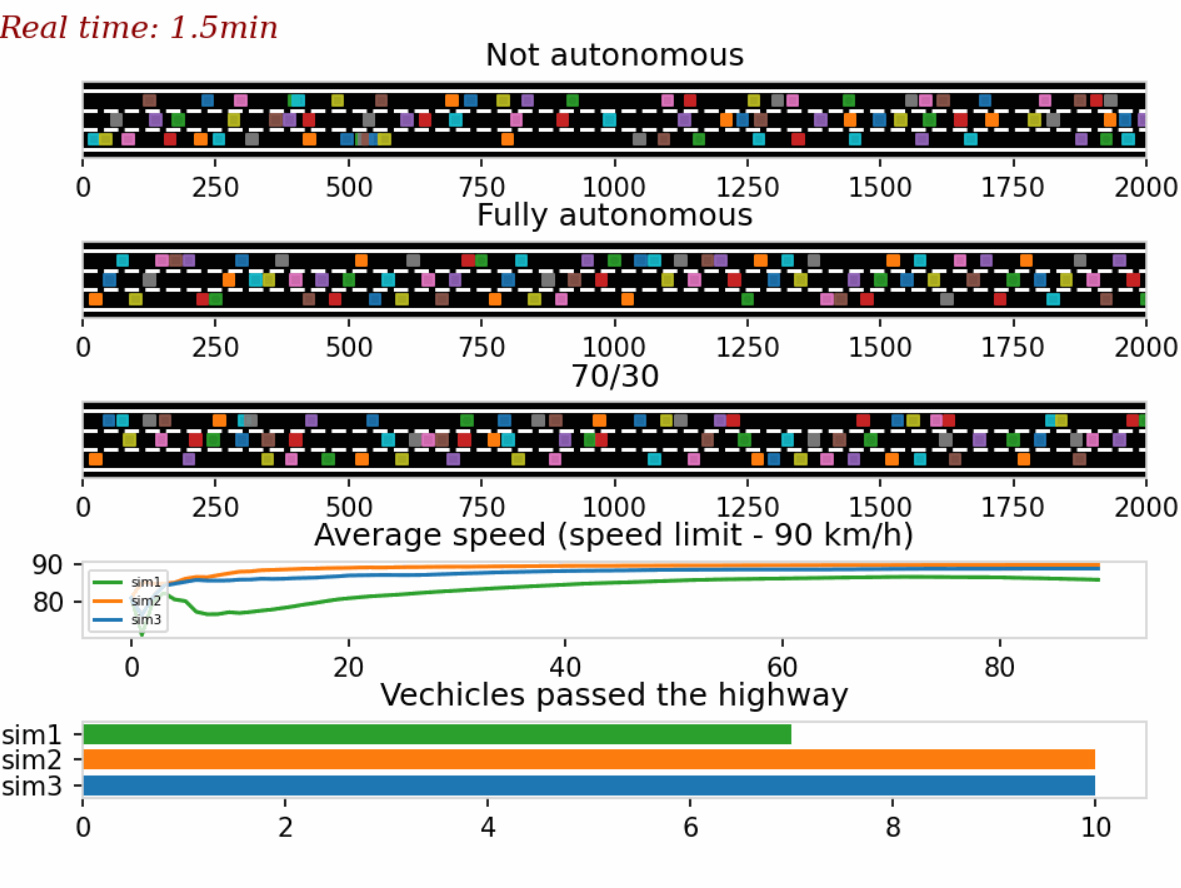
\includegraphics[width=\linewidth]{images/sim-1.png}
    \caption{Example of animation with 3 different simulations.}
    \label{fig:animtion}
\end{figure}

More detailed animation outcomes with color-coding based on a type of vehicle can be found in appendix \ref{appendix:color-output}.
\newpage
\section{Experiments Analysis}
In order to extract data out of the simulator, several experiments were run using various settings. A set of base parameters were determined for each experiment. These parameters are then adjusted to dependent on the scenario.
The base case was determined to be:
\begin{itemize}
    \item Inflow [vehicle/min] = 35 \cite{Green2020GuideTT}
    \item Simulation Time [min] = 20
    \item Average driver mood = 0.85
    \item Number of lanes = 4
    \item Highway length [km] = 10
    \item Speed limit [km/h] = 110
    \item Proportion of Autonomous cars = variable
    \item Proportion of Trucks = 0.0 % 10% normal
\end{itemize}
For all experiments, the proportion of autonomous cars were varied, to extract results 0.0 to 1.0 in 0.1 intervals. Additionally, for each of the experiments, one of the following parameters was varied based on a predetermined range. The experiment was run with varying inflow, number of lanes, speed limit, and proportion of trucks. This was done to account for the randomness factor of the simulations, since a favourable or unfavourable random seed could lead to skewed results. Furthermore, to account for the randomness factor, the simulation was run 20 times, and the average of these results was calculated. 
The experiments were run without any of the visualization described in the previous section, as it was not needed for them. Finally, for each simulation the amount of cars passing the highway (referred to as traffic flow) and the average speed of the cars were recorded. The higher the flow rate \& average speed the better. 

Running 20 simulations for each combination of two variable data points means that each experiment consist of 1200 to 2000 simulations. To speed things up, they are run concurrently using multi-threading. Even with multi-threading it took more than six hours to run all these simulations on the machine used. Some simulations, especially the ones with greater inflow and greater number of cars, require more computational time than others as multiple loops involving vehicle instances are running in the simulation.

\subsection{Experiments with varying inflow}
The experiments were done with varying inflow to show the effect different proportions of autonomous cars has on the traffic inflow. This will also show if there are specific levels of inflow, where autonomous cars have a bigger or smaller impact on the traffic flow. The inflow is varied from 10 to 60 at steps of 10. Along with the 11 different values for proportion of autonomous cars, it gives a total of 66 data points, each consisting of 20 simulations.
As we are focusing on the autonomous cars, the proportion of trucks is 0 in this experiment.

\begin{figure}[H]
    \centering
    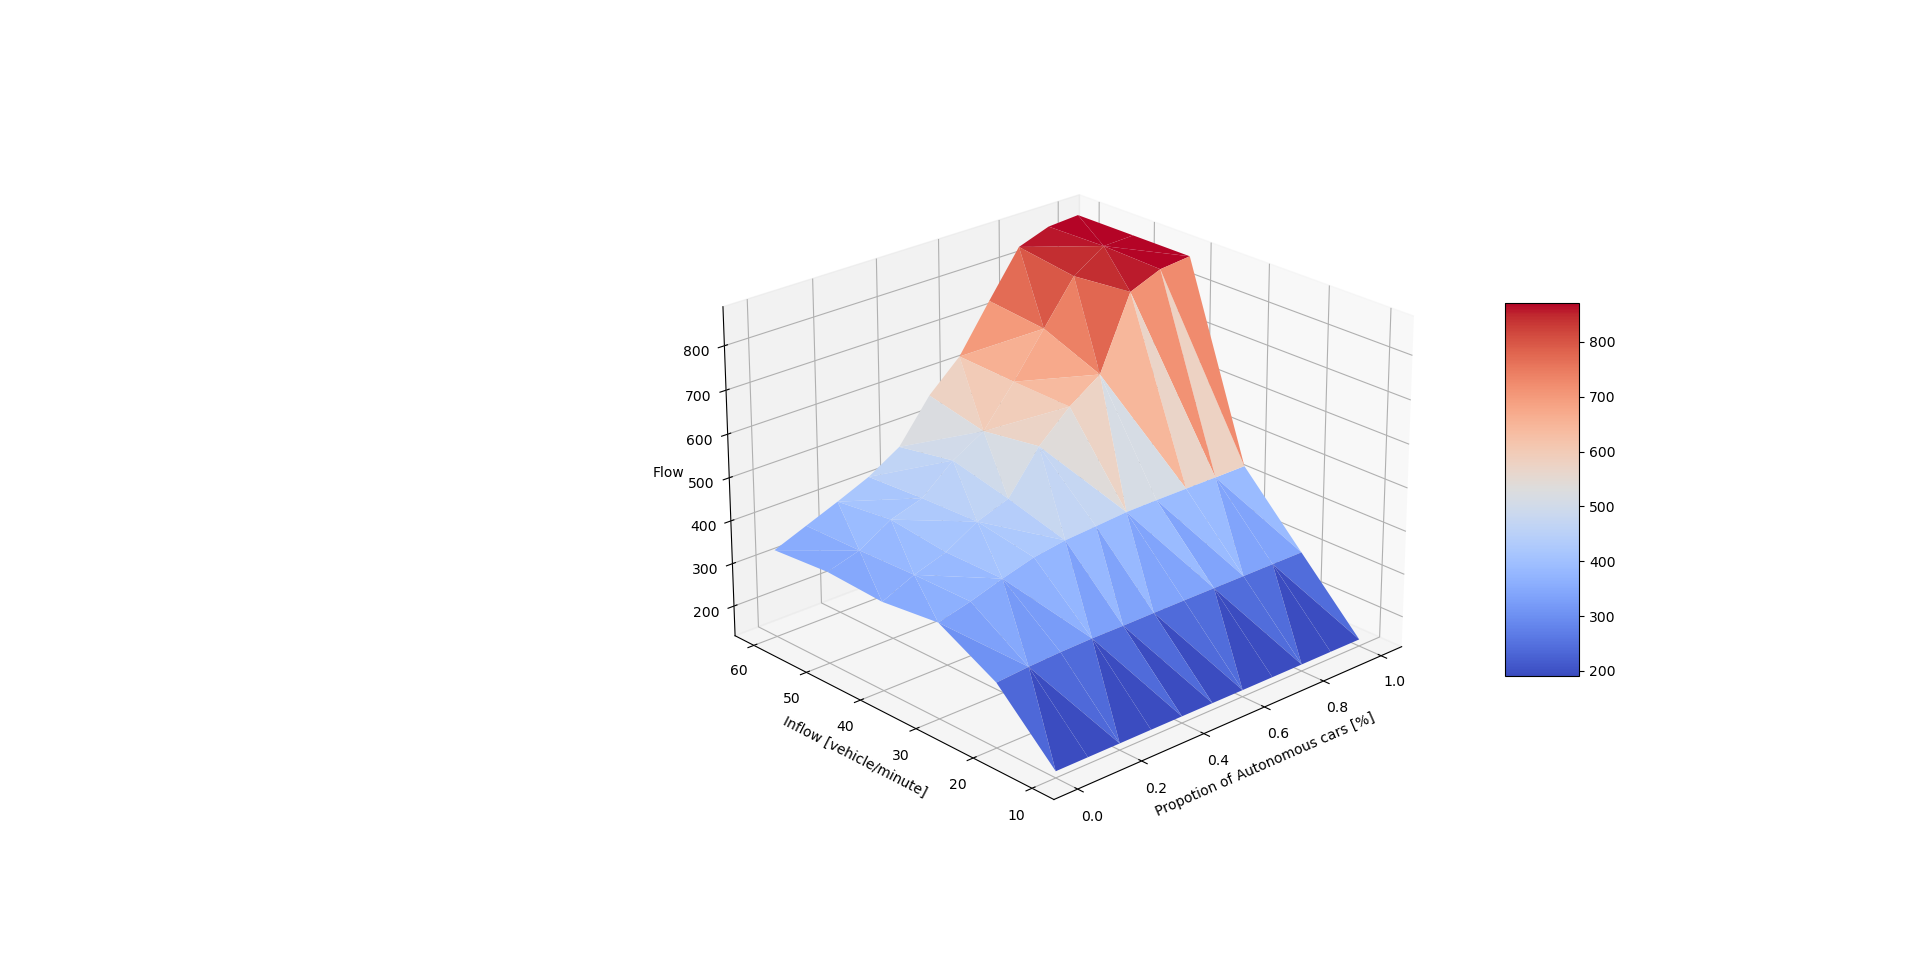
\includegraphics[width=0.5\textwidth]{images/Experiment1.png}
    \caption{Experiments with varying inflow}
    \label{fig:experiment1}
\end{figure}

The results of this experiment, which can be seen in figure \ref{fig:experiment1},  shows that at low inflow (<30), the amount of autonomous cars does not have any significant change the traffic flow. However, on higher inflow there is a close to linear correlation, where more autonomous cars means higher traffic flow. At inflow > 30, the traffic flow is more than doubled between 0\% and 100\% autonomous cars. 
\begin{figure}[H]
    \centering
    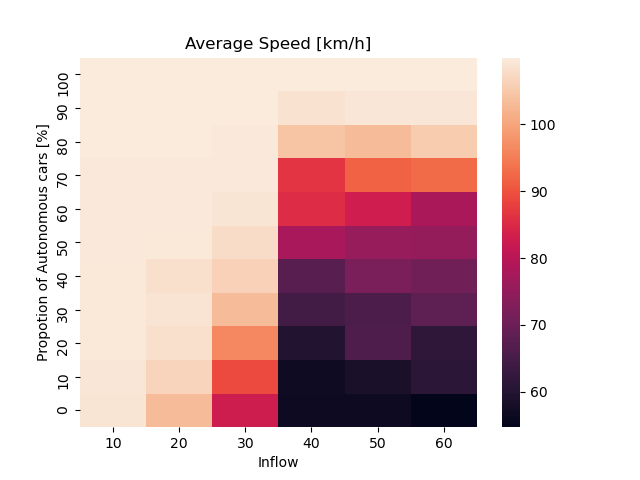
\includegraphics[width=\linewidth]{images/Experiment1-Speed.png}
    \caption{Heatmap for experiments with varying inflow}
    \label{fig:experiment1heatmap}
\end{figure}
A heatmap visualizing the average speed can be seen in figure \ref{fig:experiment1heatmap}. When looking at the average speed, the speed limit is reach fairly easily for inflow $\leq 30$, while for inflow > 30 more than 80\% autonomous cars are needed to reach the speed limit. This corresponds to the above results for traffic flow.

\subsection{Experiments with varying number of lanes}
The purpose of this experiment was to determine whether the autonomous cars needed a minimum number of lanes before they were effective, and to determine if too many lanes negates the effect of autonomous cars. The number of lanes was varied from 1 to 9 lanes, which along with the varied proportion of autonomous cars gives a total of 99 data points each consisting of 20 simulations. As we are focusing on the autonomous cars, the proportion of trucks is 0 in this experiment. 

\begin{figure}[H]
    \centering
    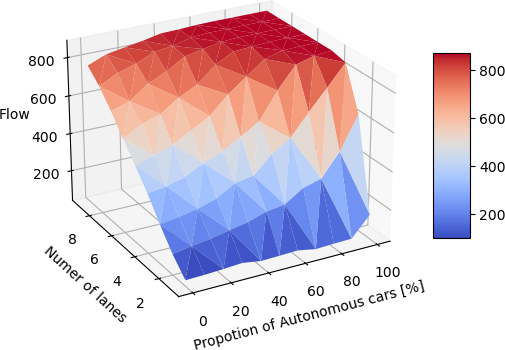
\includegraphics[width=0.5\textwidth]{images/Experiment2.png}
    \caption{Experiments with varying number of lanes}
    \label{fig:experiment2}
\end{figure}

The results of this experiment, which can be seen in figure \ref{fig:experiment2}, shows that the traffic flow hits a maximum when number of lanes, and proportion of autonomous cars increase. With 4 lanes the maximum is hit at around 80\% autonomous cars, and with more lanes  fewer autonomous cars are needed needed to  reach the max. It also shows that for autonomous cars to have any impact on the traffic  flow, at least two lanes are needed, but preferably three or more.

Similar results can also be seen when looking at the data for average speed, where a clear diagonal line is formed, indicating that more lanes and more autonomous cars are equally effective at increasing the average speed. This can be seen visualized in a heatmap in figure \ref{fig:experiment2heatmap}. 
\begin{figure}[H]
    \centering
    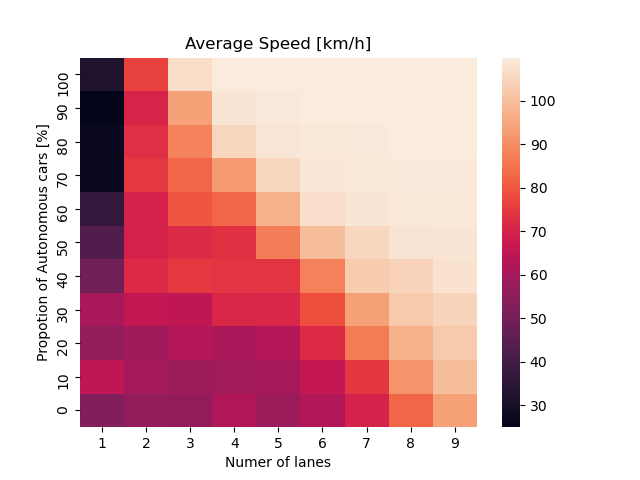
\includegraphics[width=\linewidth]{images/Experiment2-Speed.png}
    \caption{Heatmap for experiments with varying number of lanes}
    \label{fig:experiment2heatmap}
\end{figure}


\subsection{Experiments with varying speed limit}
This experiment was done to determine if changing the speed limit has an effect on the impact of autonomous cars. The speed limit is varied from 50 to 130 at 10 step intervals, along with the varied proportion of autonomous cars, it gives a total of 99 data points of 20 simulations each.  As we are focusing on the autonomous cars, the proportion of trucks is 0 in this experiment.
\begin{figure}[H]
    \centering
    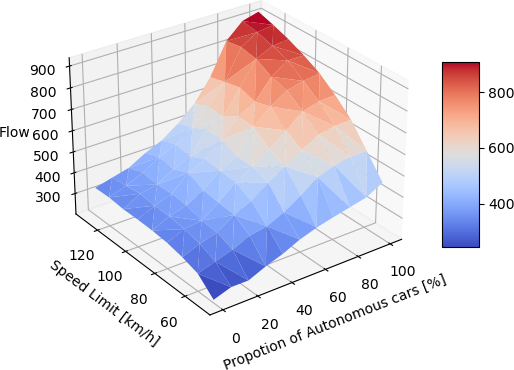
\includegraphics[width=0.5\textwidth]{images/Experiment3.png}
    \caption{Experiments with varying speed limit}
    \label{fig:experiment3}
\end{figure}
In figure \ref{fig:experiment3} the results of this experiment can be seen. This indicates that a higher speed limit increases the impact of more autonomous cars. The curve for the results with 0.0 autonomous cars quickly hits a plateau, while it gets steeper the more autonomous cars are added. 

Looking at the average speed, the results again show that more than 80\% autonomous cars, makes the average speed close the the speed limit. This is visualized as a heatmap in figure \ref{fig:experiment3heatmap}. 
\begin{figure}[H]
    \centering
    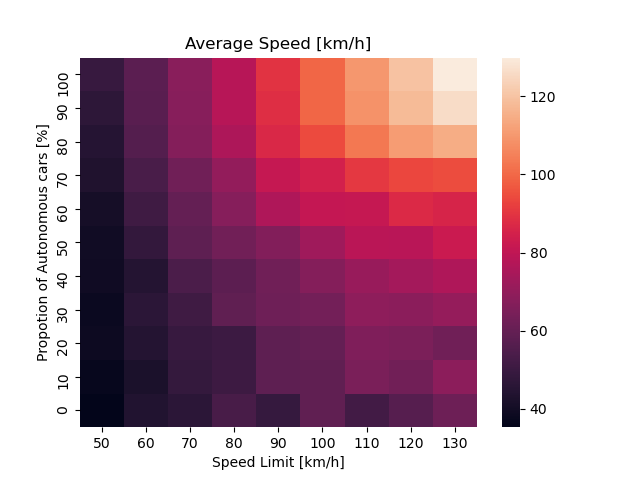
\includegraphics[width=\linewidth]{images/Experiment3-Speed.png}
    \caption{Heatmap for experiments with varying speed limit}
    \label{fig:experiment3heatmap}
\end{figure}
Both results also show that at at least 40\%-50\% autonomous cars are needed before increasing the speed limit will make any significant change to the traffic flow and average speed. This will primarily be due to this phantom traffic preventing the higher speed limit to be fully utilized.


\subsection{Experiments with varying amount of trucks}
The final experiment was done to determine what effect slow vehicles like trucks have on the impact of autonomous. This experiment limited the variables to where the sum of the two variables was less than or equal to 1. This was done because they are represented as percent of the total cars, so if the sum is more than 1, then there are more than 100\% cars.

\begin{figure}[H]
    \centering
    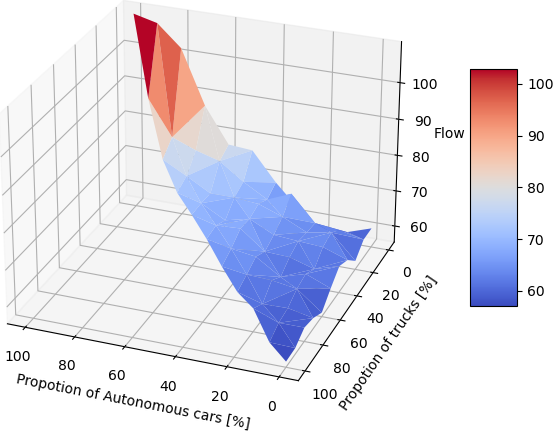
\includegraphics[width=0.5\textwidth]{images/Experiment4.png}
    \caption{Experiments with varying proportion of trucks}
    \label{fig:experiment4}
\end{figure}

The results of this experiment still shows that more autonomous cars mean higher traffic flow. It again shows the best results with more than 80\& autonomous cars, however in this case, the overall traffic flow is much lower than the other experiments, at all proportions of trucks.

%\subsection{Base experiment with no Autonomous cars}
%\subsection{Experiments with different number of Autonomous cars}
%\subsection{Experiment with only Autonomous cars}
\section{Discussion}
\subsection{Results}
The experiments that have been conducted provide a large amount of insight in whether or not it is beneficial to use V2V and autonomous driving technology. 

As seen in the analysis of the experiments, it can clearly be seen that an increase in proportion of autonomous vehicles lead to an increase in flow and higher average speed for all vehicles. It can be seen from the results in figure \ref{fig:experiment1} of the experiments, how after an 80\% proportion of autonomous vehicles, the flow and speed is nearly the optimal in a simple highway experiment. 

The results also shows that even though not 100\% of vehicles are using the autonomous and V2V communication technology, there is still a significant increase in flow of cars and the average speed of the cars. The increase is actually close to being doubled when the proportion is only 60\% 

This means that it is not necessary for everyone to be using these two technologies for there to be a benefit from it. Because of this the technology can be introduced over a longer period of time as it becomes more available to the general public to use while stile providing benefits for everyone.  

It can also be seen from the experiments in figure \ref{fig:experiment3} how that when the speed limit increases, automation of vehicles becomes even more effective compare to a regular vehicle. 
This allows for cities to increase speed limits, without worrying about accidents and traffic jams which allows people to spend less time on the road.

These results clearly indicate how autonomous vehicles would greatly improve the traffic situation on a highway with recurring traffic problems. However the results does not account for the factors which were not simulated, such as weather, roadwork and other external factors that can also have an effect on the highway. But it still shows how on a very basic level autonomous cars can increase the traffic flow of a simple highway.


\section{Conclusion}
\label{sec}
The aim of this report was to understand how V2V communication and autonomous driving, would affect traffic flow during peak hours and if it could solve the problem of phantom traffic. For that purpose, a traffic simulator was modeled and developed, it has the capability to replicate a highway environment in which different parameters can be set in order to produce a specific scenario. 
This simulator has allowed us to test the model and to study how different percentages of autonomous vehicles influence the traffic and, most importantly, it has proved that it is not necessary to have a scenario where the totality of cars are \textit{connected} to obtain relevant benefits. \\
The main tests replicate a standard highway during rush hour and the results show that with 60\% of the autonomous car the flow is doubled and around 80\% the flow almost reaches its upper limit only increasing slightly if the autonomous car parameter is brought up to 100\%. 

A visualization tool has also been created in order to produce graphical animation of how the traffic varies over time during the simulation and the real-time results. It allows the user to set up and visualize different simulations at the same time in order to have a visual comparison. 

The project resulted in a successful model that has proven to be comprehensive of complex methods such as the real-life behavior of a driver that by itself was a complex challenge. This project managed to recreate an environment in which, if the right parameter is set, it can be clearly observed the generation of phantom traffic jams due to different driving styles and different behaviors of drivers.
In the same scenario, but with the introduction of connected autonomous cars, it is clear how knowing in advance information about other vehicles and the autonomous driving capabilities prevent the creation of phantom traffic.

\subsection{Future Work}
In future works following ideas are proposed to improve the performance, functionality, and usability of the simulations system.
\subsubsection{Entry and exit lane}
The entry and exit lane is partly implemented in the current system model. Entry and exit lanes aims at creating a more realistic flow of the highway where phantom congestion can occur due to the switching lane behavior that is required of a driver when entering and exiting a highway. 
\subsubsection{Multiple vehicle classes}
Implementing different vehicle classes besides the car and truck class. Potential vehicle classes include busses and motorcycles with additional features as maximum speed limit, acceleration, and etc. 
\subsubsection{Advanced highway}
Including features aiming to create a realistic course of the highway in particular curved lanes, temporarily closed lanes and stoplights at the end of the highway which reduces the speed of the cars. Additionally, simulating scenarios with emergencies where first respond vehicles requires different driver behavior.  
\subsubsection{Algorithm for autonomous driving}
Optimize the autonomous driving of the vehicles by developing an unsupervised machine learning algorithm that trains on the simulation by evaluating the results after each run.
\subsubsection{Improved V2V communication}
Implement new parameters in the autonomous car class like error rate, range, and delay in order to have a better simulation of the V2V communication. 
\subsubsection{Vehicle caravan} 
Create a car caravan for vehicles with similar destinations thus reducing congestion caused by lane shifting and optimizing air drag however this requires a model that calculates the speed of the communication to create a minimum safe distance for the vehicles when accelerating and braking.
\subsubsection{Visualization} 
Optimize animation to improve the representation of the different vehicle classes and the separation of autonomous vehicles. Furthermore, creating a more realistic visualization of the highway.
\subsubsection{Weather} 
Including weather changes that affect the traffic flow to create a more realistic simulation model where acceleration and braking depend on the weather conditions.



\bibliographystyle{ACM-Reference-Format}
\bibliography{bibliography/bibliography} 

\clearpage

\appendix
\onecolumn
% Insert your Lean Canvas and other appendices.
\section{Scrum}
\label{appendix:appendix1}
Scrum methodology was adopted in this project. Team held weekly or biweekly scrum meeting were everybody presented his work and talked about future task. As for a software stack team was using:

\begin{itemize}
    \item Slack for communication.
    \item Slack extensions for GitHub ant trello for notifications.
    \item Github for source control.
    \item Trello for sprint tasks management.
    \item Zoom for meetings.
    \item Azure DevOps for CI/CD.
    \item Notion, google suit for project wiki.
\end{itemize}


% --------------------
\section{Code}
\label{appendix:appendix2}
\subsection{Class diagram}
\label{appendix:classDiagram}
\begin{figure}[H]
    \centering
    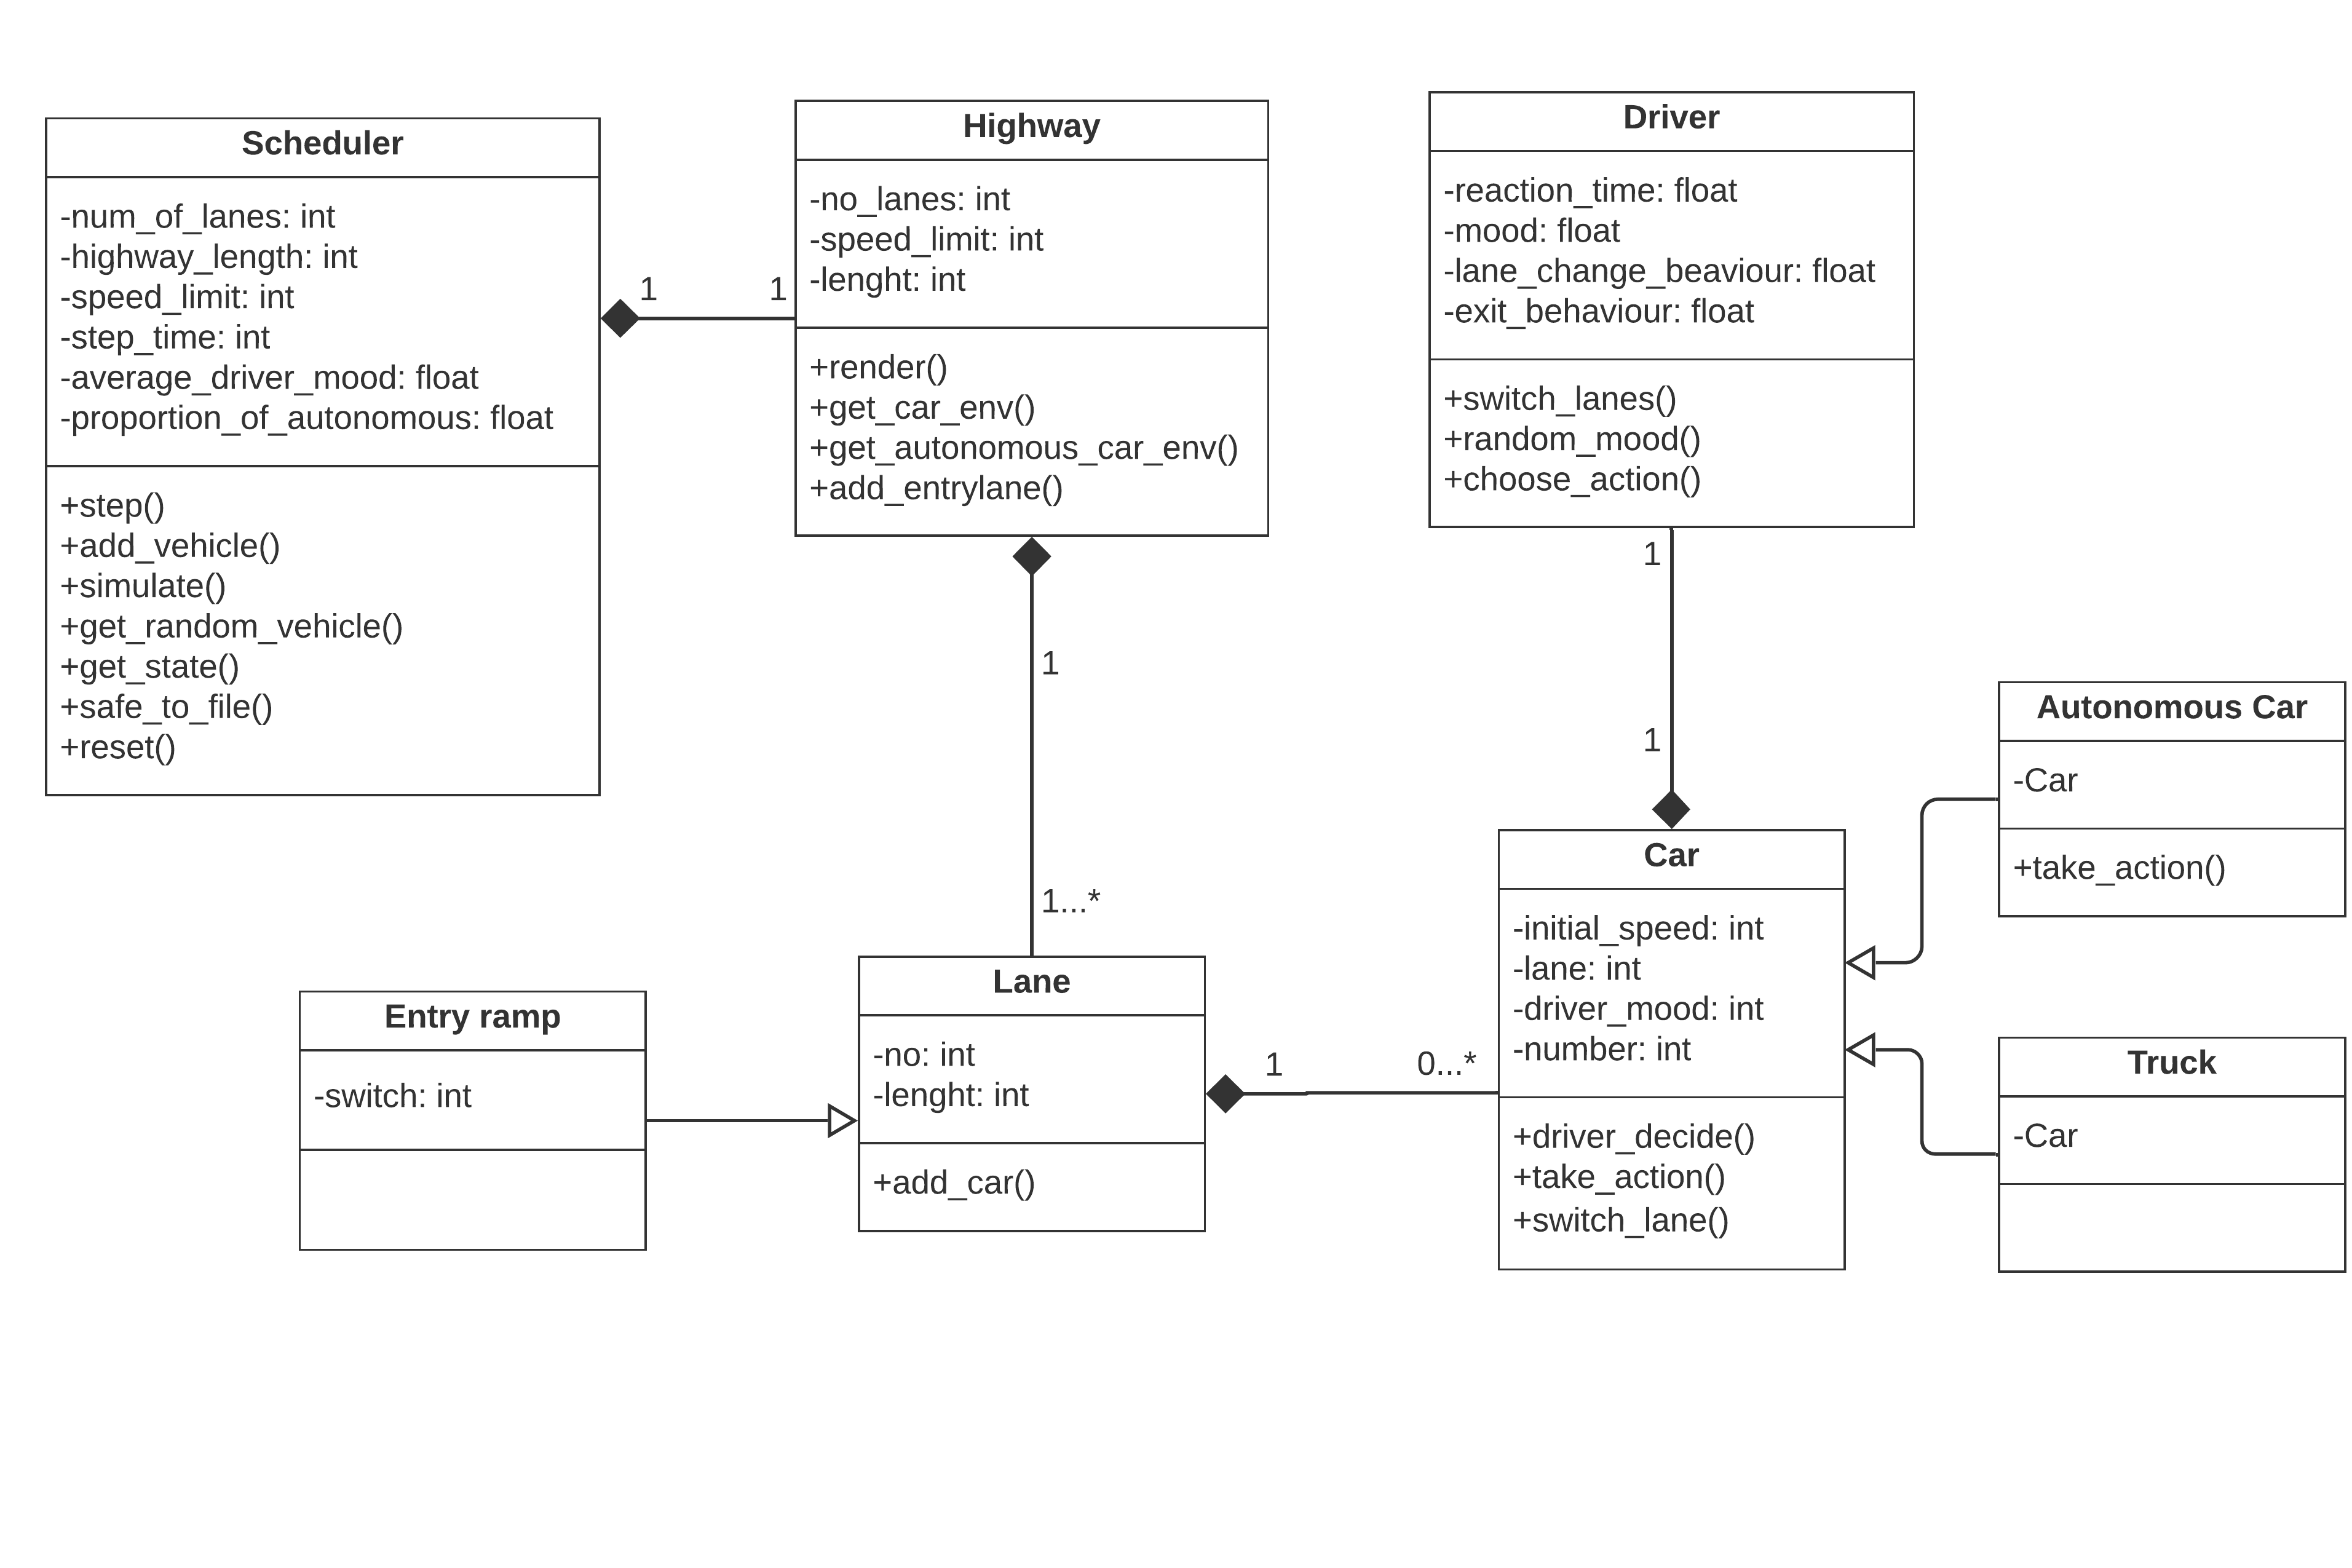
\includegraphics[width=\linewidth]{images/UML class (1).png}
    \caption{Class Diagram}
    \label{fig:classDiagram}
\end{figure}


\subsection{Testing}
Automatized testing was introduced using Azure DevOps pipelines. For every push and PR in the repository, it was tested if simulation is able to produce any result as well if there is an option to save and restore data from simulation.

\begin{figure}[H]
    \centering
    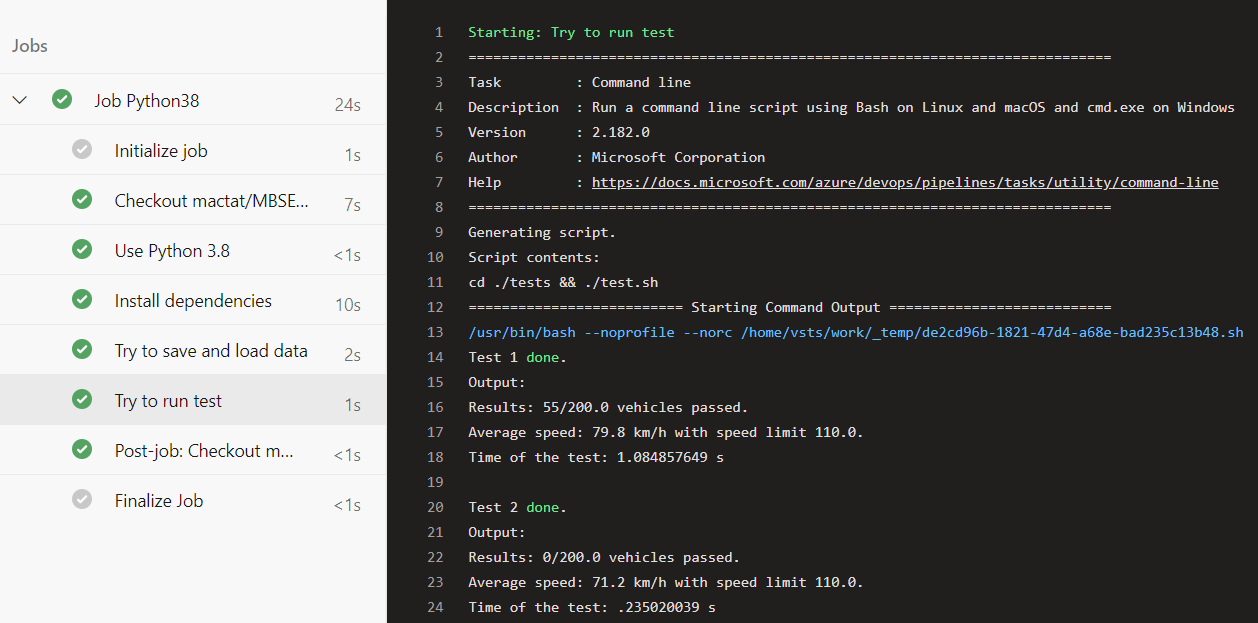
\includegraphics[width=0.8\linewidth]{images/automatic-test.png}
    \caption{Automated testing approach}
    \label{fig:automated-testing}
\end{figure}

\subsection{Output}
\label{appendix:color-output}
\begin{figure}[H]
    \centering
    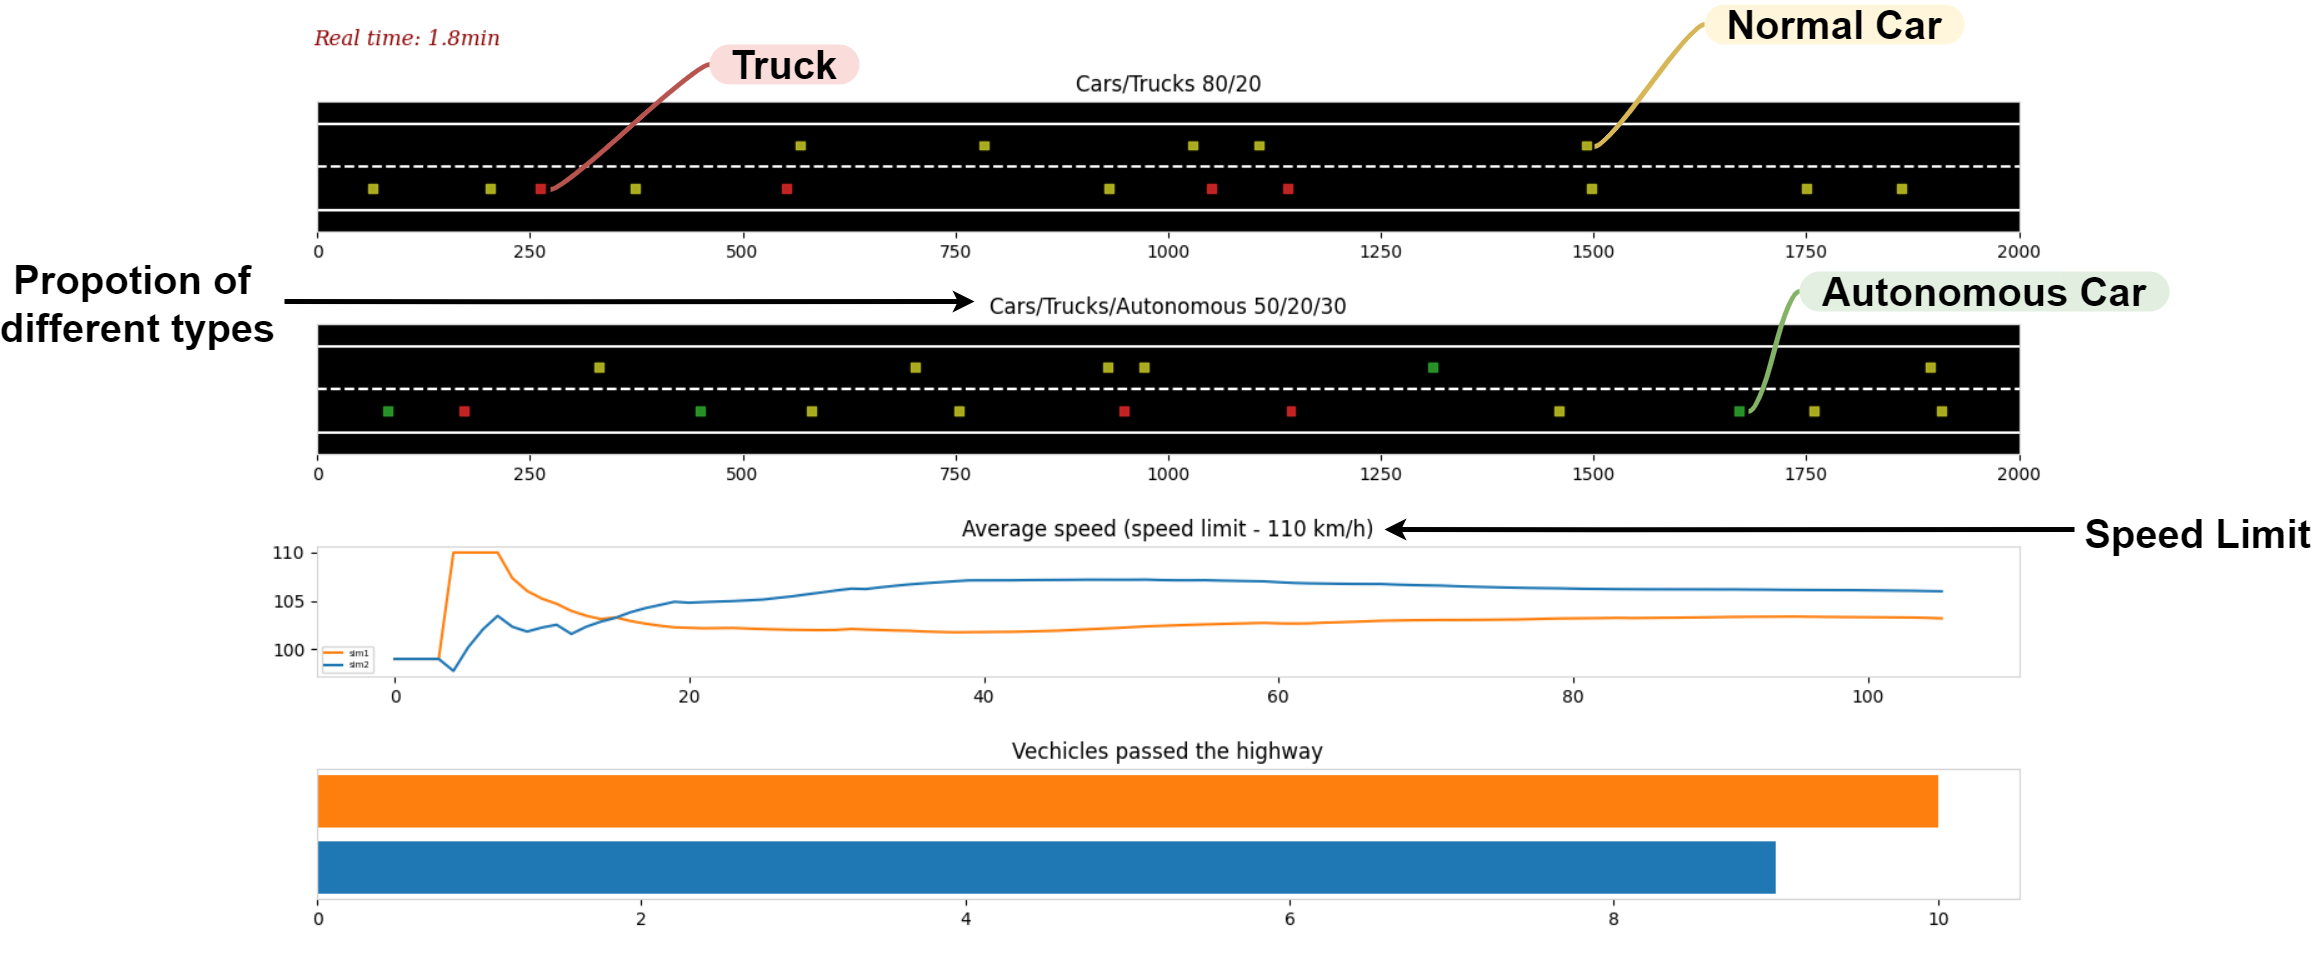
\includegraphics[width=\linewidth]{images/sim-colors-annotate.png}
    \caption{Coloring of different types of vehicles.}
    \label{fig:color-output}
\end{figure}

\section{JSON schema}
\label{appendix:json-schema}
\begin{figure}[H]
    \centering
    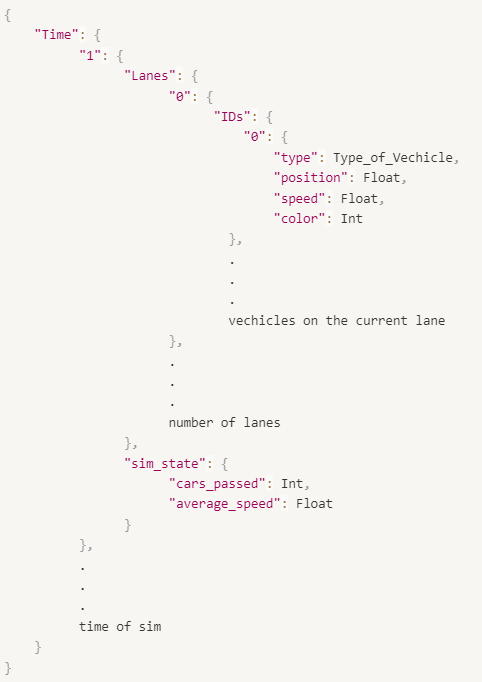
\includegraphics[width=0.5\linewidth]{images/json-schema.png}
    \caption{JSON schema}
    \label{fig:json-schema}
\end{figure}

\end{document}
